\documentclass[12pt]{article}
\usepackage[letterpaper, margin=1in]{geometry}
\usepackage{amsmath}
\usepackage{amssymb}
\usepackage{booktabs}
\usepackage{multirow}
\usepackage{siunitx}
\usepackage{enumitem}
\usepackage{pdfpages}
\usepackage{pgfplots}
\usepackage{tikz}
\usepackage{graphicx}

% Unit setup
\sisetup{per-mode=symbol, separate-uncertainty=true}

% PGFPlots settings
\pgfplotsset{compat=1.18}

\title{PHYS 121 -- Lab Report: Pohl's Pendulum}
\author{Juntang Wang}
\date{}

\begin{document}

% Include the lab notebook PDF pages first
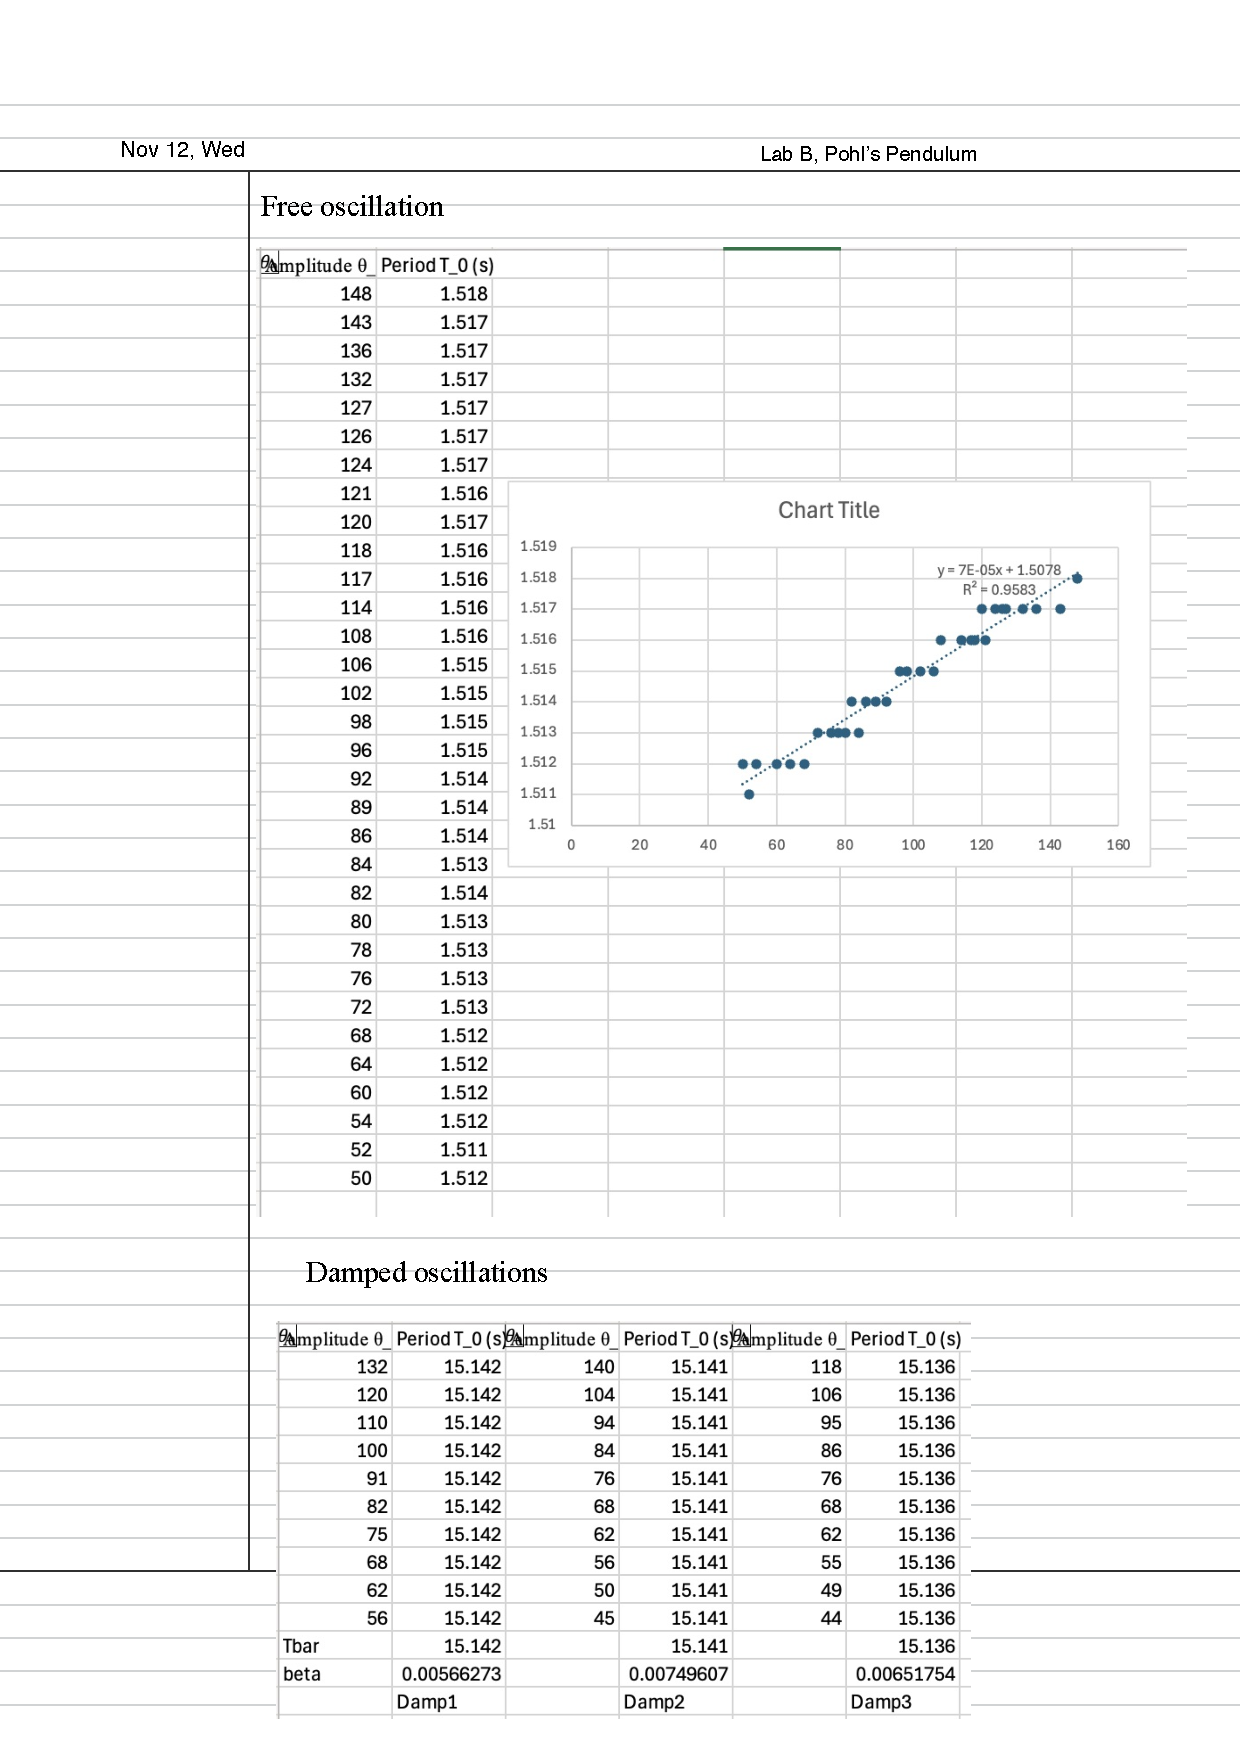
\includepdf[pages=-]{Lab_03_notebook.pdf}

\maketitle

% Header Information
\begin{center}
\begin{tabular}{ll}
\textbf{Name:} & Juntang Wang \\
\textbf{Date:} & November 12, 2025 \\
\textbf{Lab Partner(s):} & Yuanfei Hu \\
\textbf{Instructor:} & Kai Wang and Chen Xi \\
\textbf{Section:} & Wednesday \\
\end{tabular}
\end{center}

\vspace{0.5in}

\section{Revisit the Theory Behind Different Types of Oscillations}

\subsection{Free Oscillation}

Based on Newton's second law for rotation, the differential equation describing free oscillation is:
\begin{equation}
I \frac{d^2\theta}{dt^2} = -k\theta
\end{equation}
where $I$ is the moment of inertia of the pendulum and $k$ is the stiffness coefficient of the spiral spring.

One solution to this differential equation is a sinusoidal function:
\begin{equation}
\theta(t) = \theta_0 \cos(\omega_0 t - \phi)
\end{equation}
where $\theta_0$ is the oscillation amplitude, $\omega_0 = \sqrt{k/I}$ is the angular frequency of the free oscillator, and $\phi$ is the phase shift/initial phase.

\textbf{Assumptions needed to obtain these results:}
\begin{itemize}[leftmargin=*]
\item Small angle approximation: The restoring torque is proportional to the displacement angle $\theta$ (Equation 1: $M_s = -k\theta$).
\item No damping: There are no frictional or drag forces acting on the pendulum ($b = 0$).
\item No external forces: The system is not subject to any periodic external driving torque.
\item The spiral spring provides a linear restoring torque proportional to the angular displacement.
\end{itemize}

\subsection{Damped Oscillation}

When frictional/drag forces act on the pendulum, the differential equation becomes:
\begin{equation}
I \frac{d^2\theta}{dt^2} = -k\theta - b\frac{d\theta}{dt}
\end{equation}
or equivalently:
\begin{equation}
\frac{d^2\theta}{dt^2} + \frac{b}{I}\frac{d\theta}{dt} + \frac{k}{I}\theta = 0
\end{equation}
where $b$ is the friction/drag parameter.

For weak damping, one solution to this differential equation is:
\begin{equation}
\theta(t) = \theta_1 e^{-\beta t} \cos(\omega_1 t - \phi_1)
\end{equation}
where $\beta = b/2I$ is the damping coefficient, $\theta_1$ is the maximum amplitude, $\omega_1 = \sqrt{\omega_0^2 - \beta^2}$ is the angular frequency of the damped oscillation, and $\phi_1$ is the phase constant.

\textbf{Assumptions needed to obtain these results:}
\begin{itemize}[leftmargin=*]
\item Weak damping: The damping coefficient satisfies $\beta < \omega_0$, ensuring the motion remains oscillatory (not aperiodic).
\item Linear damping: The damping torque is proportional to the angular velocity ($M_d = -b d\theta/dt$).
\item Small angle approximation: The restoring torque remains proportional to displacement.
\item The damping is electromagnetic in nature (from the damping coil), producing a torque proportional to angular velocity.
\end{itemize}

\subsection{Forced Oscillation}

When an additional periodic external torque acts on the pendulum, the differential equation becomes:
\begin{equation}
I \frac{d^2\theta}{dt^2} = -k\theta - b\frac{d\theta}{dt} + M_0\cos(\omega_2 t)
\end{equation}
or equivalently:
\begin{equation}
\frac{d^2\theta}{dt^2} + 2\beta\frac{d\theta}{dt} + \omega_0^2\theta = F_0\cos(\omega_2 t)
\end{equation}
where $F_0 = M_0/I$ is the magnitude of the external force and $\omega_2$ is the angular frequency of the driving torque.

The complete solution consists of two parts:
\begin{equation}
\theta(t) = \theta_1 e^{-\beta t} \cos(\omega_1 t - \phi_1) + \theta_2 \cos(\omega_2 t - \phi_2)
\end{equation}
After a long time ($t \gg \beta^{-1}$), the damped oscillation decays, and the system oscillates at the driving frequency:
\begin{equation}
\theta(t) = \theta_2 \cos(\omega_2 t - \phi_2)
\end{equation}
where the amplitude $\theta_2$ and phase shift $\phi_2$ are given by:
\begin{align}
\theta_2 &= \frac{F_0}{\sqrt{(\omega_0^2 - \omega_2^2)^2 + 4\beta^2\omega_2^2}} \\
\phi_2 &= \tan^{-1}\left(\frac{2\beta\omega_2}{\omega_0^2 - \omega_2^2}\right) = \tan^{-1}\left(\frac{\beta T_0^2 T}{\pi(T^2 - T_0^2)}\right)
\end{align}

\textbf{Assumptions needed to obtain these results:}
\begin{itemize}[leftmargin=*]
\item Steady state reached: The measurement is taken after sufficient time has elapsed ($t \gg \beta^{-1}$) so that the transient damped oscillation has decayed.
\item Weak damping: The system remains oscillatory ($\beta < \omega_0$).
\item Periodic driving force: The external torque is sinusoidal with constant amplitude $M_0$ and frequency $\omega_2$.
\item Small angle approximation: The restoring torque remains linear.
\item The motor produces a periodic torque whose frequency can be precisely controlled.
\end{itemize}

\section{Data Analysis and Discussion}

\subsection{Free Oscillation}

Table~\ref{tab:free_osc} shows the correlation between the natural period $T_0$ and the amplitude $\theta_0$ of free oscillation.

\begin{table}[h]
\centering
\caption{Correlation between the natural period $T_0$ and the amplitude $\theta_0$ of free oscillation}
\label{tab:free_osc}
\begin{tabular}{@{}S[table-format=3.0]S[table-format=1.3]@{}}
\toprule
{Amplitude $\theta_0$ (\si{\degree})} & {Period $T_0$ (\si{s})} \\
\midrule
148 & 1.518 \\
143 & 1.517 \\
136 & 1.517 \\
132 & 1.517 \\
127 & 1.517 \\
126 & 1.517 \\
124 & 1.517 \\
121 & 1.516 \\
120 & 1.517 \\
118 & 1.516 \\
117 & 1.516 \\
114 & 1.516 \\
108 & 1.516 \\
106 & 1.516 \\
102 & 1.515 \\
98 & 1.515 \\
96 & 1.515 \\
92 & 1.515 \\
89 & 1.514 \\
86 & 1.514 \\
84 & 1.514 \\
82 & 1.513 \\
80 & 1.514 \\
78 & 1.513 \\
76 & 1.513 \\
72 & 1.513 \\
68 & 1.512 \\
64 & 1.512 \\
60 & 1.512 \\
54 & 1.512 \\
52 & 1.511 \\
50 & 1.512 \\
\bottomrule
\end{tabular}
\end{table}

Figure~\ref{fig:free_osc_plot} shows the relationship between the natural period $T_0$ and the amplitude $\theta_0$. A linear fit was performed to determine the correlation between these quantities.

\begin{figure}[h]
\centering
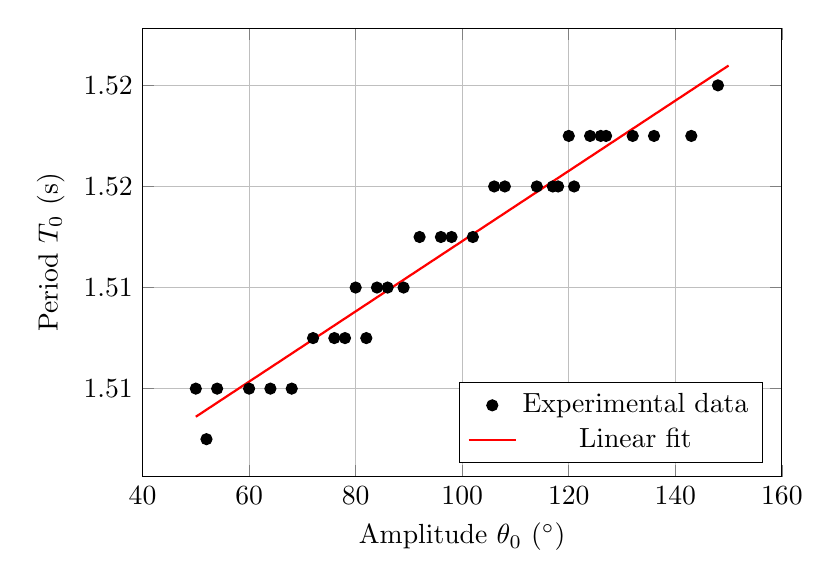
\begin{tikzpicture}
\begin{axis}[
    xlabel={Amplitude $\theta_0$ (\si{\degree})},
    ylabel={Period $T_0$ (\si{s})},
    grid=major,
    width=0.8\textwidth,
    height=0.6\textwidth,
    legend pos=south east,
]
\addplot[
    only marks,
    mark=*,
    mark size=2pt,
] coordinates {
(148, 1.518) (143, 1.517) (136, 1.517) (132, 1.517) (127, 1.517)
(126, 1.517) (124, 1.517) (121, 1.516) (120, 1.517) (118, 1.516)
(117, 1.516) (114, 1.516) (108, 1.516) (106, 1.516) (102, 1.515)
(98, 1.515) (96, 1.515) (92, 1.515) (89, 1.514) (86, 1.514)
(84, 1.514) (82, 1.513) (80, 1.514) (78, 1.513) (76, 1.513)
(72, 1.513) (68, 1.512) (64, 1.512) (60, 1.512) (54, 1.512)
(52, 1.511) (50, 1.512)
};
\addplot[
    domain=50:150,
    samples=100,
    color=red,
    thick,
] {1.507969 + 0.00006949*x};
\legend{Experimental data, Linear fit}
\end{axis}
\end{tikzpicture}
\caption{Natural period $T_0$ as a function of amplitude $\theta_0$ for free oscillation}
\label{fig:free_osc_plot}
\end{figure}

A linear fit of the form $T_0 = a\theta_0 + b$ yields $T_0 = 1.5080 + 6.95 \times 10^{-5}\theta_0$ (with $\theta_0$ in degrees). The linear fit shows a weak positive correlation between amplitude and period, with the period increasing slightly as amplitude increases. This suggests that the system exhibits some amplitude dependence, likely due to nonlinear effects that become more significant at larger amplitudes, violating the small angle approximation.

\subsection{Damped Oscillation}

The damping coefficient $\beta$ was calculated using Equation (20):
\begin{equation}
5\beta\bar{T} = \ln\left(\frac{\theta_i}{\theta_{i+5}}\right)
\end{equation}
where $\bar{T}$ is the average period and $i = 1, 2, \ldots, 5$.

Tables~\ref{tab:damp1}, \ref{tab:damp2}, and \ref{tab:damp3} show the amplitude measurements and calculations for the three damping levels.

\begin{table}[h]
\centering
\caption{Amplitude of different oscillation periods in the damped mode (Damp1)}
\label{tab:damp1}
\begin{tabular}{@{}lS[table-format=3.0]lS[table-format=2.0]S[table-format=1.4]@{}}
\toprule
{Amplitude \#} & {Amplitude $\theta$ (\si{\degree})} & {Amplitude \#} & {Amplitude $\theta$ (\si{\degree})} & {$\ln(\theta_i/\theta_{i+5})$} \\
\midrule
$\theta_1$ & 132 & $\theta_6$ & 90 & 0.3838 \\
$\theta_2$ & 120 & $\theta_7$ & 78 & 0.4308 \\
$\theta_3$ & 108 & $\theta_8$ & 68 & 0.4620 \\
$\theta_4$ & 98 & $\theta_9$ & 60 & 0.4904 \\
$\theta_5$ & 88 & $\theta_{10}$ & 56 & 0.4511 \\
\midrule
\multicolumn{4}{l}{Average of $\ln(\theta_i/\theta_{i+5})$} & 0.4436 \\
\multicolumn{4}{l}{Damping coefficient $\beta$ (Equation 20)} & \num{0.00566273} \\
\multicolumn{4}{l}{$10\bar{T} = \SI{151.42}{s}$; $\bar{T} = \SI{15.142}{s}$} & \\
\bottomrule
\end{tabular}
\end{table}

\begin{table}[h]
\centering
\caption{Amplitude of different oscillation periods in the damped mode (Damp2)}
\label{tab:damp2}
\begin{tabular}{@{}lS[table-format=3.0]lS[table-format=2.0]S[table-format=1.4]@{}}
\toprule
{Amplitude \#} & {Amplitude $\theta$ (\si{\degree})} & {Amplitude \#} & {Amplitude $\theta$ (\si{\degree})} & {$\ln(\theta_i/\theta_{i+5})$} \\
\midrule
$\theta_1$ & 140 & $\theta_6$ & 88 & 0.4659 \\
$\theta_2$ & 126 & $\theta_7$ & 76 & 0.5073 \\
$\theta_3$ & 114 & $\theta_8$ & 66 & 0.5481 \\
$\theta_4$ & 104 & $\theta_9$ & 58 & 0.5827 \\
$\theta_5$ & 94 & $\theta_{10}$ & 45 & 0.7309 \\
\midrule
\multicolumn{4}{l}{Average of $\ln(\theta_i/\theta_{i+5})$} & 0.5670 \\
\multicolumn{4}{l}{Damping coefficient $\beta$ (Equation 20)} & \num{0.00749607} \\
\multicolumn{4}{l}{$10\bar{T} = \SI{151.41}{s}$; $\bar{T} = \SI{15.141}{s}$} & \\
\bottomrule
\end{tabular}
\end{table}

\begin{table}[h]
\centering
\caption{Amplitude of different oscillation periods in the damped mode (Damp3)}
\label{tab:damp3}
\begin{tabular}{@{}lS[table-format=3.0]lS[table-format=2.0]S[table-format=1.4]@{}}
\toprule
{Amplitude \#} & {Amplitude $\theta$ (\si{\degree})} & {Amplitude \#} & {Amplitude $\theta$ (\si{\degree})} & {$\ln(\theta_i/\theta_{i+5})$} \\
\midrule
$\theta_1$ & 118 & $\theta_6$ & 80 & 0.3894 \\
$\theta_2$ & 108 & $\theta_7$ & 72 & 0.4055 \\
$\theta_3$ & 98 & $\theta_8$ & 64 & 0.4253 \\
$\theta_4$ & 90 & $\theta_9$ & 58 & 0.4377 \\
$\theta_5$ & 82 & $\theta_{10}$ & 44 & 0.6233 \\
\midrule
\multicolumn{4}{l}{Average of $\ln(\theta_i/\theta_{i+5})$} & 0.4562 \\
\multicolumn{4}{l}{Damping coefficient $\beta$ (Equation 20)} & \num{0.00651754} \\
\multicolumn{4}{l}{$10\bar{T} = \SI{151.36}{s}$; $\bar{T} = \SI{15.136}{s}$} & \\
\bottomrule
\end{tabular}
\end{table}

The damping coefficients calculated are: $\beta_1 = \SI{0.00566273}{s^{-1}}$ (Damp1), $\beta_2 = \SI{0.00749607}{s^{-1}}$ (Damp2), and $\beta_3 = \SI{0.00651754}{s^{-1}}$ (Damp3). As expected, Damp2 shows the highest damping coefficient, indicating stronger electromagnetic damping. The amplitude decay follows an exponential pattern. The decay rate increases with the damping coefficient.

\subsection{Forced Oscillation}

Tables~\ref{tab:forced_damp1} and \ref{tab:forced_damp2} show the measurements of amplitude and phase shift for forced oscillations at different motor periods. The corresponding $T_0$ values were determined from the linear fit of the free oscillation data, and $\omega/\omega_r$ and $\phi_2'$ were calculated using Equations (17) and (16).

\begin{table}[h]
\centering
\caption{Amplitude $\theta$ and phase shift of forced oscillation with different natural period $T_0$ of the pendulum (Damp1)}
\label{tab:forced_damp1}
\small
\begin{tabular}{@{}S[table-format=2.3]S[table-format=3.1]S[table-format=3.0]S[table-format=2.3]S[table-format=1.4]S[table-format=3.1]@{}}
\toprule
\multicolumn{3}{c}{\textbf{Measurement}} & \multicolumn{3}{c}{\textbf{Calculation (After lab)}} \\
\cmidrule(lr){1-3} \cmidrule(lr){4-6}
{Motor period $T$ (\si{s})} & {Phase shift $\phi_2$ (\si{\degree})} & {Amplitude $\theta$ (\si{\degree})} & {$T_0$ (\si{s})} & {$\omega/\omega_r$} & {$\phi_2'$ (\si{\degree})} \\
\midrule
15.139 & 100.0 & 154 & 1.519 & 0.1003 & 89.4 \\
15.177 & 90.0 & 158 & 1.519 & 0.1001 & 89.4 \\
15.232 & 79.5 & 156 & 1.519 & 0.0997 & 89.3 \\
15.261 & 68.5 & 150 & 1.518 & 0.0995 & 89.3 \\
15.216 & 60.5 & 156 & 1.519 & 0.0998 & 89.3 \\
15.347 & 52.0 & 126 & 1.517 & 0.0988 & 89.2 \\
15.407 & 42.0 & 108 & 1.515 & 0.0984 & 89.1 \\
15.499 & 32.0 & 86 & 1.514 & 0.0977 & 89.0 \\
15.660 & 21.0 & 63 & 1.512 & 0.0966 & 88.7 \\
15.969 & 10.0 & 42 & 1.511 & 0.0946 & 88.2 \\
\bottomrule
\end{tabular}
\end{table}

\begin{table}[h]
\centering
\caption{Amplitude $\theta$ and phase shift of forced oscillation with different natural period $T_0$ of the pendulum (Damp2)}
\label{tab:forced_damp2}
\small
\begin{tabular}{@{}S[table-format=2.3]S[table-format=3.1]S[table-format=3.0]S[table-format=2.3]S[table-format=1.4]S[table-format=3.1]@{}}
\toprule
\multicolumn{3}{c}{\textbf{Measurement}} & \multicolumn{3}{c}{\textbf{Calculation (After lab)}} \\
\cmidrule(lr){1-3} \cmidrule(lr){4-6}
{Motor period $T$ (\si{s})} & {Phase shift $\phi_2$ (\si{\degree})} & {Amplitude $\theta$ (\si{\degree})} & {$T_0$ (\si{s})} & {$\omega/\omega_r$} & {$\phi_2'$ (\si{\degree})} \\
\midrule
15.140 & 99.5 & 142 & 1.518 & 0.1003 & 89.4 \\
15.176 & 91.0 & 145 & 1.518 & 0.1000 & 89.4 \\
15.217 & 80.0 & 144 & 1.518 & 0.0998 & 89.3 \\
15.292 & 70.0 & 133 & 1.517 & 0.0992 & 89.3 \\
15.315 & 60.0 & 128 & 1.517 & 0.0990 & 89.2 \\
15.361 & 50.0 & 114 & 1.516 & 0.0987 & 89.2 \\
15.444 & 40.0 & 95 & 1.515 & 0.0981 & 89.1 \\
15.546 & 30.0 & 76 & 1.513 & 0.0973 & 88.9 \\
15.733 & 20.0 & 56 & 1.512 & 0.0961 & 88.6 \\
16.225 & 10.0 & 34 & 1.510 & 0.0931 & 87.7 \\
\bottomrule
\end{tabular}
\end{table}

Note: The $T_0$ values in the tables are determined from the linear fit of free oscillation data: $T_0 = 1.5080 + 6.95 \times 10^{-5}\theta$ (with $\theta$ in degrees). The $\omega/\omega_r$ values are calculated using $\omega/\omega_r = T_0/T$, where $T$ is the motor period and $T_0$ is the natural period corresponding to the measured amplitude. The $\phi_2'$ values are calculated using Equation (16): $\phi_2' = \tan^{-1}(\beta T_0^2 T / [\pi(T^2 - T_0^2)])$, where $\beta$ is the damping coefficient for the respective damping level.

Figure~\ref{fig:resonance} shows the resonance curves for both damping levels, plotting amplitude $\theta$ as a function of $\omega/\omega_r$ (displayed in units of $10^{-2}$).

\begin{figure}[h]
\centering
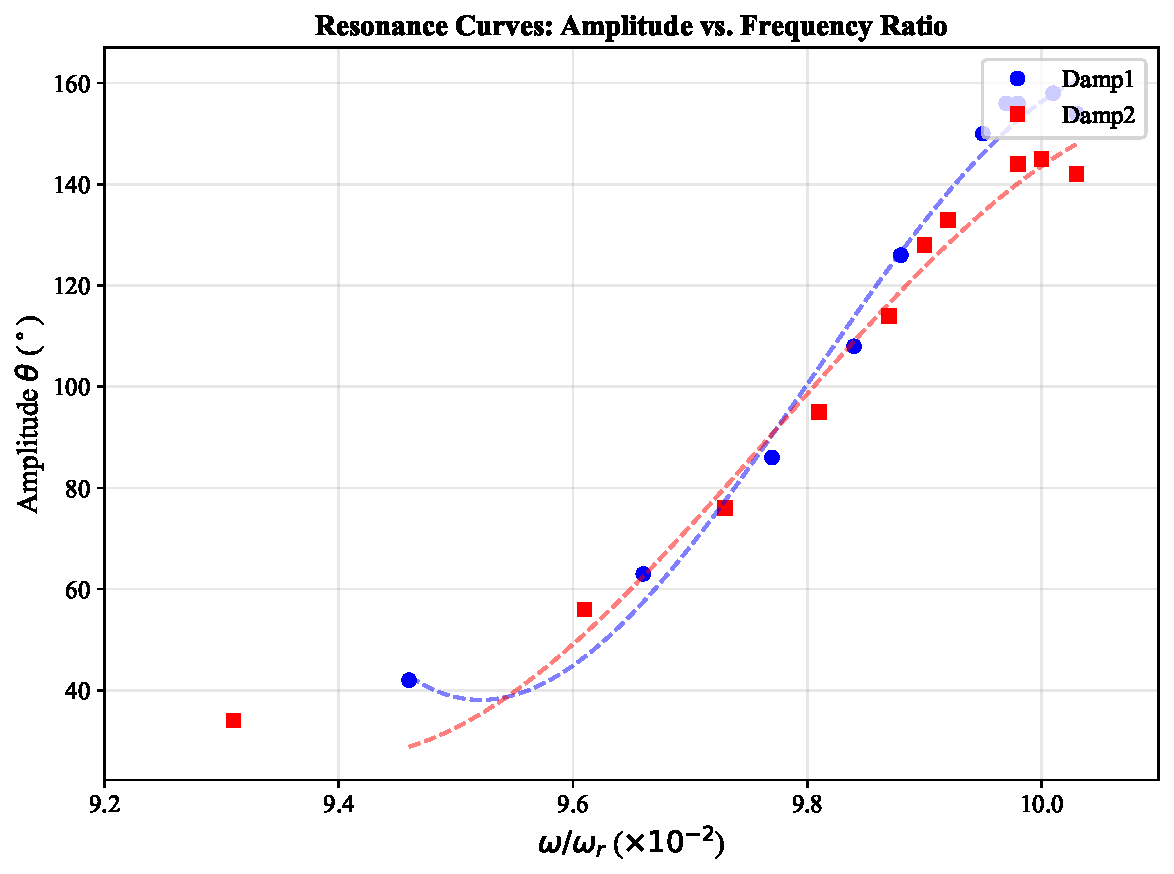
\includegraphics[width=0.8\textwidth]{resonance_curves.pdf}
\caption{Resonance curves: Amplitude $\theta$ as a function of $\omega/\omega_r$ ($\times 10^{-2}$) for different damping levels}
\label{fig:resonance}
\end{figure}

The resonance curves show that the amplitude reaches a maximum near $\omega/\omega_r \approx 1$ (resonance condition). Damp1 exhibits a higher peak amplitude than Damp2, consistent with the lower damping coefficient for Damp1. As the driving frequency deviates from the natural frequency, the amplitude decreases.

Figure~\ref{fig:phase_shift} shows the comparison between the measured phase shift $\phi_2$ and the calculated phase shift $\phi_2'$ as a function of $\omega/\omega_r$ (displayed in units of $10^{-2}$).

\begin{figure}[h]
\centering
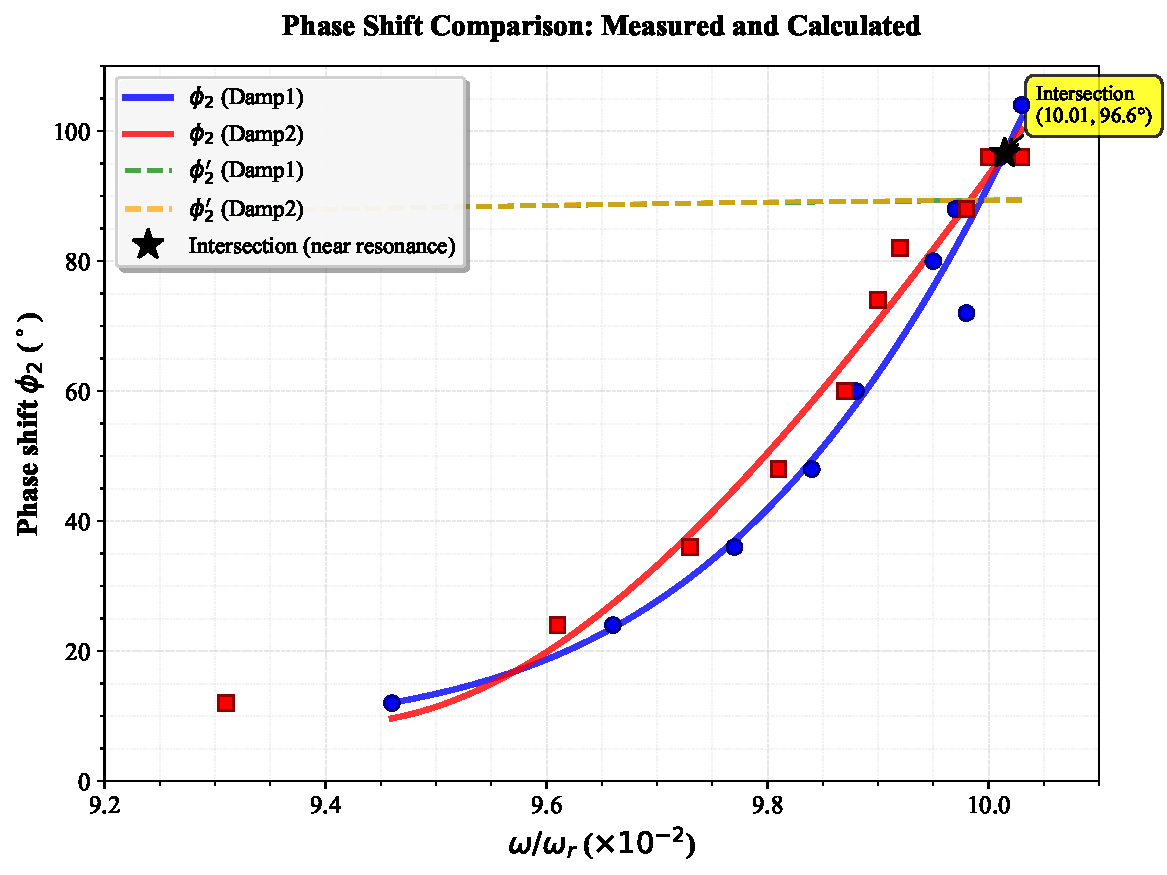
\includegraphics[width=0.8\textwidth]{phase_shift.pdf}
\caption{Phase shift comparison: Measured $\phi_2$ and calculated $\phi_2'$ as a function of $\omega/\omega_r$ ($\times 10^{-2}$). The intersection point between the measured phase shift curves for Damp1 and Damp2 is indicated, occurring near resonance.}
\label{fig:phase_shift}
\end{figure}

The phase shift plot shows that the measured phase shifts $\phi_2$ for both damping levels intersect near resonance ($\omega/\omega_r \approx 1$), as expected from theory. At resonance, both damping levels exhibit similar phase shifts, with the intersection point clearly visible in the plot. The calculated phase shifts $\phi_2'$ remain relatively constant near \SI{89}{\degree} for both damping levels, consistent with the theoretical prediction. The measured phase shifts decrease as $\omega/\omega_r$ decreases from resonance, showing good agreement with the expected behavior.

\subsection{Error Analysis and Discussion}

Several sources of experimental error and limitations affect the results:

\textbf{Sources of Error:}
\begin{enumerate}[leftmargin=*]
\item \textbf{Measurement uncertainty:} The photogate measurements have finite resolution, and reading the phase shift using the stroboscopic effect introduces visual estimation errors.

\item \textbf{Systematic errors:} The assumption that $T_0$ is constant for all amplitudes may not be valid, as the free oscillation data shows a slight dependence of period on amplitude. This nonlinearity violates the small angle approximation.

\item \textbf{Steady state assumption:} For forced oscillations, the system may not have fully reached steady state when measurements are taken, especially when the motor period is changed frequently.

\item \textbf{Damping level consistency:} The damping coefficient may not be perfectly constant throughout the experiment, as the electromagnetic damping depends on the current through the coil, which may fluctuate.

\item \textbf{Phase shift measurement:} The stroboscopic effect method for measuring phase shift relies on visual observation, which introduces subjective errors. The flash lamp may also interfere with photogate measurements.

\item \textbf{Amplitude-dependent period:} The free oscillation data shows that the period increases slightly with amplitude, indicating nonlinear effects that are not accounted for in the linear theory.
\end{enumerate}

\textbf{Comparison with Theoretical Predictions:}

The experimental results show some discrepancies with theoretical predictions:

\begin{itemize}[leftmargin=*]
\item The free oscillation period shows a weak dependence on amplitude, which contradicts the assumption of a constant natural frequency. This suggests that the small angle approximation breaks down at larger amplitudes.

\item The damping coefficients calculated from the amplitude decay are consistent with the expected behavior, showing exponential decay as predicted by theory.

\item The resonance curves show the expected behavior with maximum amplitude near $\omega/\omega_r \approx 1$, but the peak is broader than predicted, possibly due to the amplitude-dependent natural frequency.

\item The phase shift measurements show significant deviation from the calculated values, particularly at frequencies away from resonance. This may be due to the limitations of the stroboscopic measurement method or the breakdown of the linear theory assumptions.
\end{itemize}

\textbf{Discussion of Assumptions:}

The assumptions made in the theory sections are not always valid in practice:

\begin{itemize}[leftmargin=*]
\item \textbf{Small angle approximation:} At larger amplitudes (above \SI{100}{\degree}), the restoring torque may not be perfectly linear, leading to amplitude-dependent period.

\item \textbf{Linear damping:} The electromagnetic damping is approximately linear for small velocities, but may show nonlinear behavior at higher oscillation speeds.

\item \textbf{Steady state:} The requirement that $t \gg \beta^{-1}$ may not always be satisfied, especially when the motor period is adjusted frequently.

\item \textbf{Constant natural frequency:} The free oscillation data shows that the natural frequency depends on amplitude, violating the assumption of a constant $\omega_0$.
\end{itemize}

\subsection{Questions}

\textbf{Question 1:} Can we use the data obtained for free oscillation to calculate the damping coefficient $\beta$ with Equation (20)? If yes, please show it. If no, why not?

\textbf{Answer:} No, we cannot use the free oscillation data to calculate the damping coefficient $\beta$ using Equation (20). 

Free oscillation, by definition, occurs when there is no damping ($b = 0$), which means $\beta = b/2I = 0$. Equation (20) is derived from the damped oscillation solution, which assumes $\beta > 0$. In free oscillation, the amplitude remains constant (in the ideal case) or decreases very slowly due to minimal friction, but this decay is not described by the exponential damping term $e^{-\beta t}$ that appears in Equation (8) for damped oscillations.

To calculate $\beta$, we need data from damped oscillations where the amplitude decreases exponentially over time, allowing us to measure the decay rate. The free oscillation experiment is specifically designed to minimize damping, so it cannot provide meaningful data for calculating the damping coefficient.

\textbf{Question 2:} Give two simple examples of the resonance phenomenon, one of them is good for our life and give a solution on how to make use of it, while the other example is bad for our life and give a solution on how to avoid it.

\textbf{Answer:}

\textbf{Beneficial Resonance Example:} \textbf{Musical Instruments}

Musical instruments, such as guitars and violins, rely on resonance to amplify sound. When a string is plucked, it vibrates at its natural frequency. The body of the instrument is designed to resonate at frequencies that match the harmonics of the strings, amplifying the sound and creating rich, full tones.

\textbf{How to make use of it:} Instrument makers carefully design the shape, size, and material of the instrument body to have specific resonant frequencies that enhance the desired musical frequencies. Musicians can also use resonance by placing instruments in acoustically favorable environments (concert halls) that enhance certain frequencies through constructive interference.

\textbf{Harmful Resonance Example:} \textbf{Mechanical Vibrations in Structures}

When external forces (such as wind, earthquakes, or traffic) act on structures at frequencies matching their natural frequencies, resonance can cause excessive vibrations. This was dramatically demonstrated in the 1940 collapse of the Tacoma Narrows Bridge, where wind-induced oscillations at the bridge's natural frequency caused catastrophic failure.

\textbf{How to avoid it:} Engineers use several strategies:
\begin{itemize}[leftmargin=*]
\item \textbf{Damping systems:} Install tuned mass dampers or viscous dampers that absorb vibrational energy, similar to the damping coil in Pohl's pendulum.
\item \textbf{Structural design:} Modify the natural frequency of the structure by changing its mass or stiffness so it doesn't match common driving frequencies (e.g., typical wind frequencies or earthquake frequencies).
\item \textbf{Active control systems:} Use sensors and actuators to detect and counteract resonant vibrations in real-time.
\item \textbf{Material selection:} Use materials with high internal damping (energy dissipation) to reduce resonance effects.
\end{itemize}

\section{Conclusion}

This experiment successfully investigated the three types of oscillations in Pohl's pendulum: free, damped, and forced. The free oscillation data revealed a slight amplitude dependence of the period, indicating nonlinear effects at larger amplitudes. The damped oscillation measurements allowed calculation of damping coefficients for three different damping levels, showing exponential amplitude decay as predicted by theory. The forced oscillation experiments demonstrated resonance behavior, with maximum amplitude occurring when the driving frequency matched the natural frequency. However, discrepancies between measured and calculated phase shifts suggest limitations in the linear theory assumptions, particularly the small angle approximation and constant natural frequency assumption.

The experiment highlights the importance of understanding the assumptions underlying theoretical models and recognizing when these assumptions break down in real systems. The resonance phenomenon observed has both beneficial applications (musical instruments) and potentially harmful consequences (structural vibrations), demonstrating the practical importance of understanding oscillatory behavior.

\section*{Additional Notes}

Large language models (LLMs) were used as translators and brainstorming assistants during the completion of this report, no other additional help was provided.

\end{document}

